\documentclass[10pt, aps,twocolumn, superscriptaddress, nofootinbib]{revtex4-2}
%\documentclass[aps,twocolumn,floatfix, showpacs, superscriptaddress]{revtex4-2}
\usepackage[pdftex]{graphicx}% Include figure files
 \usepackage{amsmath}
\usepackage[T1]{fontenc}
\usepackage{amssymb}
\usepackage{amsfonts}
\usepackage{bm}
\usepackage{booktabs}
\usepackage{cellspace}%
\setlength\cellspacetoplimit{3pt}
\setlength\cellspacebottomlimit{3pt}
\usepackage{makecell}
 \usepackage{amsmath} 
  \usepackage{flushend}
\usepackage[breaklinks=true,colorlinks=true,linkcolor=blue,urlcolor=blue,citecolor=blue]{hyperref}
\usepackage{color}
\usepackage{longtable}
\usepackage{amsfonts} 
\usepackage{amssymb, mathrsfs}
\usepackage{braket}
\usepackage{graphicx} 
\usepackage{diagbox}
\usepackage{subfigure}
\usepackage{bbm}
\begin{document}

\date{\today}
\title{A/B Testing and Statistical Power Analysis}
\author{S. A. Owerre}
\affiliation{Data Insights and Analytics}
\email{alaowerre@gmail.com}

\begin{abstract}
In this  report, I jot down my  thoughts on A/B testing and statistical power analysis focusing mainly on the statistics behind them. In addition, I explore parametric t-tests and non-parametric tests.  This report is compiled  based on my research in this subject by reading different textbooks, papers, and blogs. 
\end{abstract}

\maketitle

\section{A/B Testing}

Suppose we want to know if adding a new feature $X$ in some e-commerce webpage will increase revenue. To do this, we randomly split users (i.e., customers) into two groups. We expose one group to the existing webpage without the new feature $X$, and the other group to the existing webpage with the new feature $X$.  Users assigned to the existing webpages with and without the new feature $X$ are called the treatment and control groups respectively as shown in Fig.~\eqref{fig1}. A user should consistently see the same webpage during the course of the experiment, to guarantee that the observations in the treatment and control groups are independent \cite{s1}.

In practice, power analysis should be conducted first to determine the minimum sample size needed to detect a particular effect size. This will be discussed in later sections. It is also recommended to start with small number of subjects (e.g. users) and increase it over time, in case something goes wrong and you need to abort the experiment abruptly. 

 \begin{figure}[ht]
    \centering
    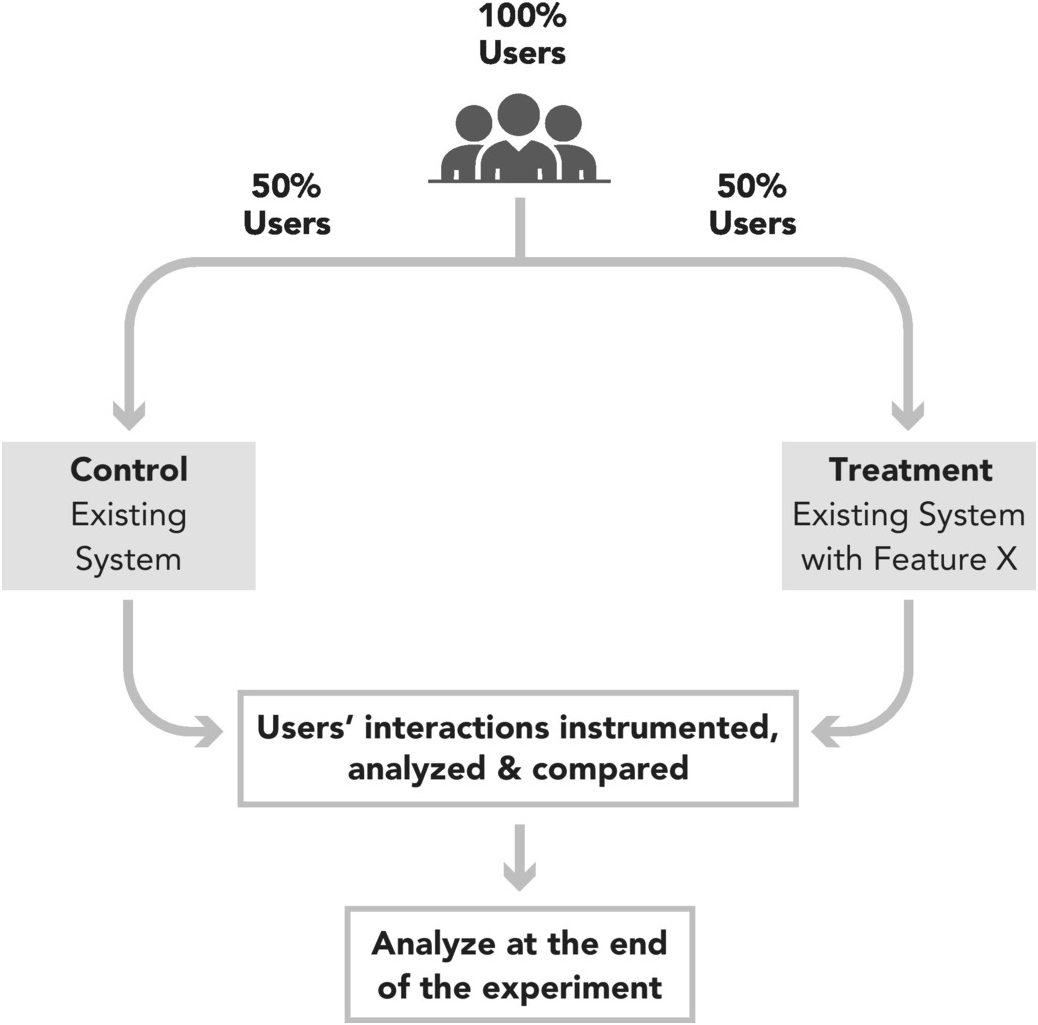
\includegraphics[scale=.8]{fig.png}
    \caption{A simple controlled experiment: An A/B Test. Adapted from Ref.~\cite{s1}.}
    \label{fig1}
\end{figure}

Assuming everything goes well and we collect data for the revenue per user generated in each group (say, after about one week). In this case, the revenue per user is our overall evaluation criterion or the metric of success. It is also called the target or dependent variable.   Usually, we assume that the treatment and control samples are drawn independently from two normally distributed populations with equal variances (or without equal variances). This leads to a two-sample t-test which will be described in later sections. 

To test the effectiveness of the new feature $X$, we can formulate the following two hypotheses:
\begin{equation}
	H_0: \mu_1 = \mu_2 \quad \text{versus}\quad H_1: \mu_1 \neq \mu_2,
	\label{eqn1}
\end{equation}
  where $\mu_1, \mu_2$ are the population means. The hypotheses in Eq.~\eqref{eqn1} are called a two-tailed (nondirectional) or a two-sided hypothesis testing. We call $H_0$ the null hypothesis and $H_1$ the alternative hypothesis. The null hypothesis states that there is no difference between the two population means, whereas the alternative hypothesis states that there is a difference between the two population means.
  
   Evidently, the hypothesis makes a statement about the population parameters. The goal of a hypothesis test is to decide, based on samples drawn from the populations (in this case the treatment and control samples), which of two complementary hypotheses is true \cite{s2}.  In hypothesis testing, there are two types of errors that can happen as shown in Table.~\eqref{tab1}: 
 
\begin{table}[ht]
 \caption{Outcomes of hypothesis testing}
 \label{tab1}
\centering
    \begin{tabular}{l|cc|}
    {} &  {Accept $H_0$ } &{Reject $H_0$} \\  
    \toprule
    {$H_0$ true} &  {\checkmark } &{type I error} \\  \midrule
   $H_1$ true  & {type II error } &{\checkmark } \\  \midrule
    \end{tabular}
    \end{table}
\begin{enumerate}
	\item {\bf type I error}  is to reject $H_0$, when it is in fact true.  This means concluding  there is a significant difference between treatment and control, when there is none.
	\item  {\bf type II error} is to accept  $H_0$, when it is in fact false. This means concluding  there is no significant difference between treatment and control, when there is one.
\end{enumerate}

    
For any test, the probability of making type I error is denoted by $\alpha$, and it is identical to the significance level, usually set at $0.05$, implying that  it is acceptable to have a 5\% probability of committing type I error.  The probability of making type II error is denoted by $\beta$ \cite{s3,s4}. Mathematically, 
\begin{align}
	\mathcal{P}(\text{rejecting}~H_0\lvert H_0~\text{true})&= \alpha,\\
	\mathcal{P}(\text{accepting}~H_0\lvert H_1~\text{true}) &= \beta.
\end{align}


\section{P-Value}

In hypothesis testing, one of the crucial questions one usually asks is: does our data provide enough evidence for us to reject the null hypothesis $H_0$  \cite{s33}? This question is usually answered with the help of the p-value.  The p-value is a measure of the evidence against the null hypothesis $H_0$: the smaller the p-value, the stronger the evidence against $H_0$. 
 Formally, the p-value is the probability of observing a test statistic at least as extreme as what was  observed, assuming that the null hypothesis is true. 

Suppose we have set a fixed significance level $\alpha$, if the probability associated with an observed value of a statistical test (under $H_0$) is less than or equal to $\alpha$, i.e, 
\begin{equation}
	\text{p-value} \leq \alpha,
\end{equation}
then we reject $H_0$ at level $\alpha$.   Such an observed value  is said to be ``statistically significant''. 
It is important to note that a large p-value $>\alpha$ is not a strong evidence in favour of $H_0$. A large p-value can occur for two reasons: $(i)$ $H_0$ is true or $(ii)$  $H_0$ is false, but the test has low power \cite{s3}. In this case (i.e., p-value $>\alpha$), it is safe to say that there is not enough data to reach any conclusion.  

\section{Interference or Network effect}
\subsection{Interference Problem}
Most controlled experiments rely upon the fact that the Stable Unit Treatment Value Assumption (SUTVA) holds \cite{su, su2}. This states that the outcomes of any unit (user) in the experiment is unaffected by variant assignment of other units. In other words, the outcome of any  unit in the experiment is not affected by the treatment of any other  unit. The potential outcome of interest  if SUTVA holds is 
\begin{align}
Y_i({\bf Z}) = Y_i(Z_i),
\end{align}
where ${\bf Z} \in \lbrace 0,1\rbrace^N$ is the treatment vector of units,  $i\in \lbrace 1,2,3,\cdots, N\rbrace$ such that $Z_i =1$ if unit $i$ receives a treatment and $Z_i =0$ if unit $i$ receives the control (no treatment). 

Running A/B testing experiments in social networks (such as Facebook, LinkedIn, etc.) can lead to a violation of SUTVA, because each user is by design connected to other users. The violation of SUTVA is called network effect or interference.

 For instance, suppose Facebook introduced a new feature to increase user engagement with WhatsApp; a user in the treatment group is likely to send more messages to other users in her network that may be in the control group, who then send more messages back as  they reply. If the success metric is the total number of messages sent, then both treatment and control total messages are likely to increase, therefore the metric would be biased and leads to inaccurate estimates of the treatment effect.

\subsection{Solutions and Challenges}

One way to mitigate interference is to first identify the medium connecting the treatment and control groups. Once identified, a common solution is to use cluster-based randomization assignment. This is usually done by constructing a graph with units as nodes and edges are their connections (e.g., followers or friends). The treatment or control is now assigned to clusters or communities (connected subgraph) in the graph rather than individual units.  Some of the challenges of this approach  include:
\begin{enumerate}
 \item  Isolated communities are difficult to achieve. 
 \item To increase the power of the test we need more clusters (communities), but the larger the number of clusters the less isolated they are.

\end{enumerate}


\section{Parametric T-Tests}
The t-test is {\it parametric} in that it makes assumptions on the population distributions (or the parameters of the populations) from which the samples were drawn.  The meaningfulness of the result of a t-test depends on the validity of the assumptions. Thus,  before using a particular t-test,  it is advisable to examine if the assumptions that a test is based upon is valid using the sample data. Here, I will discuss the commonly used t-tests: the Student's t-test and the Welch's t-test.

\subsection{The Student's T-Test}
In the development of  two-sample Student's t-test, we make the following assumptions:
\begin{enumerate}
	\item \textit{Normality}: The two samples are assumed to be drawn from two normally distributed populations with unknown variances or standard deviations. To test this assumption in practice, one should plot the histogram of each sample to see if it follows a normal distribution especially when the sample size is large enough. If the distribution is right skewed, a log transformation can be applied. However, performing t-test on the log transformed data can be difficult to interpret since you cannot map the result back to the untransformed data unlike in regression analysis.
	
	
	\item \textit{Equal variances}: The two populations are assumed to have equal variance, i.e.,  homoscedasticity. To test this assumption  requires an examination of the variance of each sample. If the sample variances are roughly the same, then it is reasonable to assume that they are estimating a common population variance. In this case, we can pool the two sample variances as the estimate of the population common  variance. 
	
	\item \textit{Independence}: The two samples are assumed to be drawn independently. This assumption is tested by the experimenter when designing the experiment. The experimenter should make sure that during the course of the experiment each subject (randomization unit) is assigned to either the treatment or the control to avoid repeated measurement from the same subject. In other words, a subject cannot generate an observation in both the treatment and the control.  This guarantees that there is no relationship between the observations in one group as compared to the other.  Therefore, each unit's assignment to a particular variant  $Z_i (i = 1,2,\cdots, N)$ is a Bernoulli random variable
	\begin{align}
	Z_i = \text{Bernoulli}(p),
	\end{align}
	with probability of assignment to a particular variant $p$.
\end{enumerate}

Formally, let $x_1^i \sim \mathcal{N}(\mu_1, \sigma_1^2),~i = 1,2,\cdots, n_1$; and  $x_2^i \sim \mathcal{N}(\mu_2, \sigma_2^2), ~i = 1,2,\cdots, n_2$, where $x_1^i$ and $x_2^i$ are independent, and  $\sigma_1^2 = \sigma_2^2 = \sigma^2$ with $\sigma$ unknown.  We can think of the samples $x_1$'s and $x_2$'s as observations from the treatment and control groups respectively.  The test statistic is defined as
  \begin{equation}
 	t^* =\frac{\bar{x}_1 -\bar{x}_2}{SE({\bar{x}_1 -\bar{x}_2})},
 	\label{eqn8}
 \end{equation}
 where  $\bar{x}_1$ and $\bar{x}_2$ are the two sample means (i.e., the estimates of $\mu_1$ and $\mu_2$), and $SE({\bar{x}_1 -\bar{x}_2})$ is the  standard error of $\bar{x}_1 -\bar{x}_2$, given by
  \begin{align}
 	SE({\bar{x}_1 -\bar{x}_2}) &= \sqrt{\frac{s_{\text{pooled}}^2}{n_1} + \frac{s_{\text{pooled}}^2}{n_2}},\nonumber\\&
 	=s_{\text{pooled}}\sqrt{\frac{n_1+n_2}{n_1n_2}},
 	\label{eqn9}
 \end{align} 
 where $s_{\text{pooled}}^2$ is the sample pooled variance (i.e., the estimate of the common population variance $\sigma^2$) given by
 \begin{equation}
 	s_{\text{pooled}}^2 = \frac{(n_1-1)s_1^2 + (n_2-1)s_2^2}{n_1+n_2-2},
 	\label{pool}
 \end{equation} 
 where $n_1, n_2$ are the two sample sizes, and $s_1^2, s_2^2$ are the two sample variances, given by
 \begin{equation}
 	s_i^2 = \frac{1}{n_i-1}\sum_{j=1}^{n_i}(x_j - \bar{x}_i)^2,\quad i = 1, 2.
 	\label{vars}
 \end{equation}
  
 \begin{figure}[ht]
    \centering
    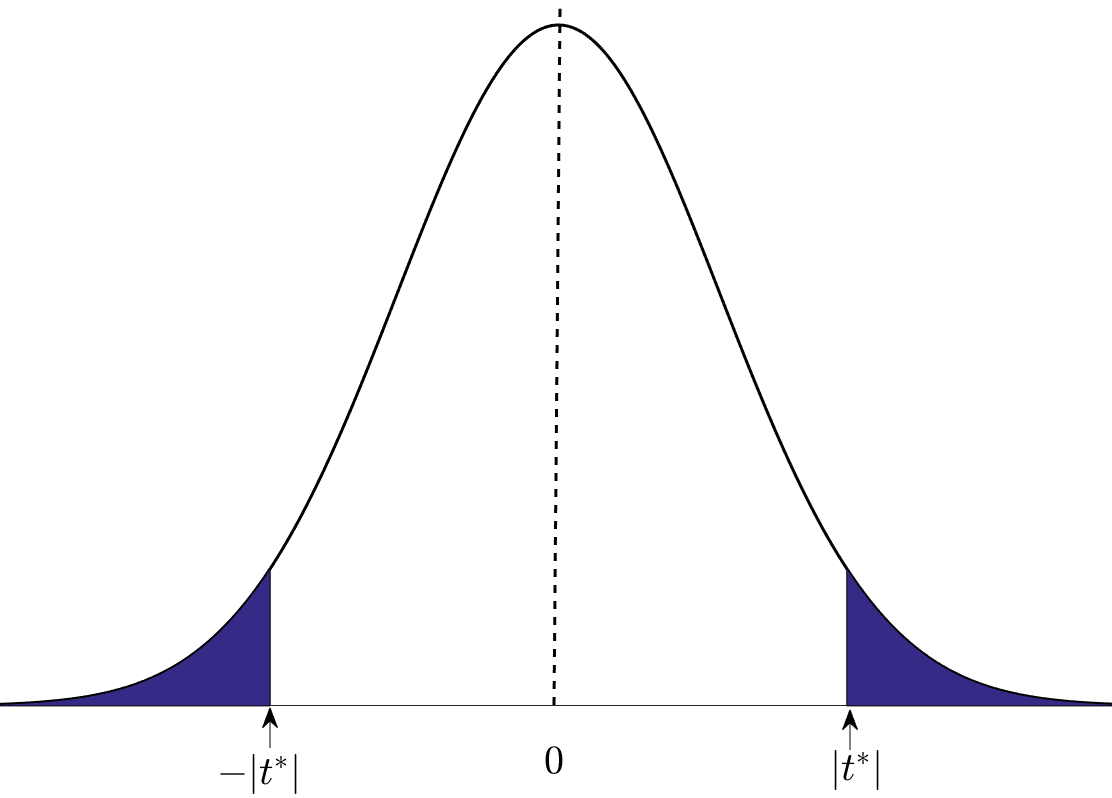
\includegraphics[scale=.2]{t_dist.png}
    \caption{A plot of the t-distribution (under $H_0$) for sample size $\nu = 50$. The area under the shaded regions is the p-value. }
    \label{fig2}
\end{figure}

The test statistic $t^*$ measures the number of standard deviations that $\bar{x}_1-\bar{x}_2$ is away from the null hypothesis $\mu_1-\mu_2 = 0$.  Assuming that the null hypothesis is true, the probability of observing any value equal to $|t^*|$ or large is the p-value. To compute this p-value, we need to know the sampling distribution of $t^*$,  that is, if we repeatedly draw random samples of equal size from the populations under $H_0$, and compute $t^*$ for each sample drawn.  What is its distribution?   The distribution is the Student's t-distribution  given by \cite{s3a,s3s}
 \begin{equation}
 f_\nu(t) = \frac{\Gamma\left(\frac{\nu+1}{2}\right) }{\sqrt{\nu\pi}\Gamma\left(\frac{\nu}{2}\right)}\Big( 1+\frac{t^2}{\nu}\Big)^{-\frac{\nu +1}{2}}
  \end{equation}
where $\nu$  is the number of degrees of freedom.

The test-statistic  $t^*$ is drawn from the t-distribution with $\nu=n_1+n_2-2$ degrees of freedom, and for large samples, i.e., $\nu\to \infty,~f_\nu(t)\to \mathcal{N}(0,1)$.  The p-value is the area of the two shaded regions in Fig.~\eqref{fig2}, given by
 \begin{align}
 \text{p-value} &= \mathcal{P}\Big(|T| \geq |t^*| \Big\vert T = f_\nu(t) \Big) \nonumber\\&
 = \mathcal{P}\Big(T \leq -|t^*|~\text{or}~T \geq |t^*| \Big\vert T = f_\nu(t) \Big)\nonumber \\&
 = 2\mathcal{P}\Big(T \leq -|t^*|  \Big\vert T = f_\nu(t)\Big) \nonumber \\&= 2{\Phi}_\nu\big(-|t^*|\big),
   \end{align}
 where ${\Phi}_\nu(x)$  is the cumulative distribution function (CDF) of the t-distribution.
 
 The $100(1-\alpha)\%$ confidence interval for $\delta = \mu_1-\mu_2$ is given by
\begin{align}
 \hat{\delta} - t^*_{\nu, \alpha/2}SE(\hat{\delta} ) \leq \delta  \leq\hat{\delta}  + t^*_{\nu, \alpha/2}SE(\hat{\delta} )
 \end{align}
where $\hat{\delta}  = \bar{x}_1-\bar{x}_2$ and $ t^*_{\nu, \alpha/2}$   is a critical value of $t^*$ with $\nu =n_1+n_2-2$ degrees of freedom. 

If the confidence interval does not contain zero, it means that the null hypothesis $\delta =0$ is false and we reject it. Therefore, $\hat{\delta}$ is statistically significant at level $\alpha$ if the $100(1-\alpha)\%$ confidence interval  does not contain zero, which is equivalent to $\text{p-value} < \alpha$. Note that for large sample sizes $(\nu \to \infty)$ and $\alpha =0.05$, the critical value  $ t^*_{\nu \to \infty, 0.025}\approx 1.96$, so $\delta$ is about 2-standard deviation away from $\hat{\delta}$ on both sides.

\subsection{The Welch's T-Test}

The assumption of equal variances in the Student's t-test is not always tenable. In this case, the distribution of the test statistic is no longer a t-distribution. This is called the Behrens-Fisher problem \cite{s3b}. The Welch approximation for this problem is called the Welch's t-test \cite{s3c}. Suppose $\sigma_1^2\neq \sigma_2^2$ and both population variances are unknown, the test-statistic is given by
\begin{equation}
 	t^\prime =\frac{\bar{x}_1 -\bar{x}_2}{SE({\bar{x}_1 -\bar{x}_2})},
 	\label{eqn8a}
 \end{equation}
 where  $SE({\bar{x}_1 -\bar{x}_2})$ is now given by
  \begin{align}
 	SE({\bar{x}_1 -\bar{x}_2}) &= \sqrt{\frac{s_{1}^2}{n_1} + \frac{s_{2}^2}{n_2}},
 	\label{eqn99}
 \end{align} 
where  $s_1^2, s_2^2$ are the two sample variances in Eq.~\eqref{vars}, which are the estimates of the two unequal  population variances. The exact distribution of $t^\prime$ is  very complex. However,   it can be approximated to a t-distribution with $\nu$ degrees of freedom,  given by

\begin{equation}
	\nu \approx \frac{\Big(\frac{s_1^2}{n_1} + \frac{s_2^2}{n_2}\Big)^2}{\frac{s_1^4}{n_1^2(n_1-1)} + \frac{s_2^4}{n_2^2(n_2-1)}}.
\end{equation}
Note that $\nu$ is generally non-integer unlike the Student's degrees of freedom. 

\subsection{Summary of Procedure for T-Test }
In this section, I summarize the steps that should be taken when conducting a t-test. Given an experimental data, the following steps can be performed:
\begin{enumerate}

\item Verify the assumptions that the test is based upon.
\item State the two complementary hypotheses.
\item Pick a significance level, $\alpha$.
\item Compute the test statistic.
\item  Find the degrees of freedom, $\nu$.
\item Compute the p-value and compare it to  $\alpha$.
\item State the conclusion of the test results.
\end{enumerate}

{\it Programming package}:  In principle, the statistical analyses of t-test can be coded manually. However, it is advisable to use programming softwares especially for large data. In this regard, the Python  SciPy package  \href{https://docs.scipy.org/doc/scipy/reference/generated/scipy.stats.ttest_ind.html}{scipy.stats.ttest\_ind} can be used to compute test statistic and its p-value  for the Student's t-test, and for Welch's t-test set the equal\_var parameter to False.

\section{Non-parametric Tests}
In the {\it parametric} t-test, assumptions are made in advance about the population distributions. However, in some instances these assumptions may not be valid.   It is often difficult to have access to normally distributed samples. When the data do not meet the normality and (un)equal variance assumptions of the two-sample t-tests,   a {\it non-parametric} statistical test is recommended. For {\it non-parametric} tests, the population distributions from which the samples were drawn are not assumed in advance. Therefore, they are ``distribution-free'' \cite{s4}. 

\subsection{The Mann-Whitney U Test}
The Mann-Whitney U test is  a {\it non-parametric} test that can be used in this scenario to compare two  groups, which are assumed to be independent \cite{s4,s6,s7, s8}. In this case, the null hypothesis $H_0$ states that the two independent samples come from the same population, whereas the alternative hypothesis $H_1$ states that the two independent samples come from different populations.

 Suppose we have  $n_1$ observations $x_1^i (i=1,2,\cdots,n_1)$ in one sample (i.e. from one population) and $n_2$ observations $x_2^i (i=1,2,\cdots,n_2)$ in another sample (i.e., from another population). The Mann‐Whitney test is based on the comparison of each observation $x_1^i$ from sample 1 with each observation $x_2^i$ from  sample 2. This means that the data (sample 1 \& sample 2 combined) must be sorted in ascending order  and each observation is indexed from 1 to $N=n_1+n_2$.  If two or more observations are the same, the indexes (ranks) of those observations should be the average of the indexes. The total number of pairwise comparisons that can be made is $n_1n_2$.  
 
 If the samples have the same median then each $x_1^i$ has an equal chance (i.e., probability $1/2$) of being greater or smaller than each $x_2^i$. Hence, the hypotheses can be formally stated as
 \begin{align}
	H_0: \mathcal{P}\big(x_1^i > x_2^j\big) =\frac{1}{2}~\text{versus}~ H_1: \mathcal{P}\big(x_1^i > x_2^j\big) \neq \frac{1}{2}.
	\label{eqnu}
\end{align}
The Mann-Whitney U statistic is defined as
\begin{align}
U_1 &= n_1n_2 + \frac{ n_1(n_1+1)}{2} - R_1,\\
U_2 &= n_1n_2 + \frac{ n_2(n_2+1)}{2} - R_2,
\end{align}
where  $R_1$ is the sum of the ranks  assigned to sample 1 (i.e., sum of the indexes assigned to the observations after sorting the combined samples), and $R_2$ is the sum of the ranks assigned to sample 2. Here, $U_1$  is the  number of times an  $x_1^i$ from sample 1 is greater than an  $x_2^i$ from sample 2. Similarly,  $U_2$  is the  number of times an  $x_1^i$ from sample 1 is smaller than an  $x_2^i$  from sample 2. The sum of the ranks of the two samples is given by
 \begin{equation}
 (R_1+R_2) = 1+2+3+\cdots+N= \frac{N(N+1)}{2}.
 \end{equation}
 One can check that $U_1+U_2 = n_1n_2$, hence once either $U_1$ or $U_2$ is found, the other one can be calculated from the addition rule. 

Now define $U=\text{min}(U_1,U_2)$. The distribution of $U$ under $H_0$ has been found by Mann \& Whitney,  and the probabilities for small values of $n_1,n_2$ have a table known as the Mann-Whitney U tables. If one finds that the probability $\mathcal{P}\big(U=\text{min}(U_1,U_2)\big)<\alpha$, then the null hypothesis ($H_0$) is rejected at level $ \alpha$.

\subsubsection {Normal Approximation} 
In most A/B testing experiments, the obtained samples sizes are usually large (i.e., $n_1n_2 >20$). In this case, a normal approximation can be used by defining:
 \begin{align}
	\mu_U &= \frac{n_1n_2}{2},\quad \sigma_U =\sqrt{ \frac{n_1n_2(N+1)}{12}},
	\label{tt}
\end{align}
where $\mu_U$  and $\sigma_U$ are the mean and standard deviation of  the $U$ distribution respectively.  The corresponding test statistic is given by
 \begin{align}
	z = \frac{U -\mu_U}{\sigma_U},
\end{align}
where $z\sim \mathcal{N}(0,1)$. In the normal approximation, the computation of $U$ can be done by either $U_1$ or $U_2$,  because $|z|$ is the same whether  $U_1$ or $U_2$ is used in computing $U$.

The p-value  is calculated from the standard normal distribution under $H_0$, given by
\begin{align}
	\text{p-value} &= \mathcal{P}\Big(|Z|\geq |z|\Big\vert Z = \mathcal{N}(0,1)\Big)\nonumber\\&
	= 2\mathcal{P}\Big(Z< -|z|\Big\vert Z = \mathcal{N}(0,1)\Big) \nonumber\\&
	= 2\Phi(-|z|),
\end{align}
where $\Phi$ is the CDF of normal distribution.
\begin{enumerate}	
\item{\it Dealing with ties}: When two or more observations have the same value, it is called a tie. If the ties occur between  two or more observations in the same sample, the value of $U$ is unaffected. However, if the ties occur between  two or more observations in both  samples, the value of $U$ is affected. In this case, the standard deviation is renormalized as
\begin{align}
 \sigma_U =\sqrt{\Big(  \frac{n_1n_2}{N\big(N-1\big)}\Big)\Big(  \frac{N^3 -N}{12} - \sum_{j}^{n_s}\frac{t_j^3-t_j}{12}\Big) },
 \label{rtt}
\end{align}
where $n_s$ is the number of samples in which ties occur, and $t_j$ is the number of observations tied for a given rank in sample $j$. We can see that in the absence of ties (i.e., $t =0$), Eq.~\eqref{rtt} reduces to $\sigma_U$ in Eq.~\eqref{tt}.

\item{\it Programming package}: The  Python SciPy package \href{https://docs.scipy.org/doc/scipy/reference/generated/scipy.stats.mannwhitneyu.html}{scipy.stats.mannwhitneyu} can be used  to compute the Mann-Whitney U statistic and its p-value.
\end{enumerate}		
 
\section{Power analysis}
\subsection{Definition}
The power of a statistical test is the probability that the test correctly rejects the null hypothesis, when the alternative  hypothesis is true. In other words, it is the probability of not making the type II error.  It is also stated as the probability of detecting a treatment effect, when the effect is really there. Mathematically, 
\begin{align}
	\text {Power} =  \mathcal{P}(\text{rejecting}~H_0| H_1~\text{true})= 1-\beta.
\end{align}

It is common to conduct power analysis before starting an experimental design, to determine the (minimum) sample size needed to detect a given effect size. The use of post hoc power analysis, that is,  after the experiment has been conducted and found to be nonsignificant (say, p-value $> \alpha$), is discouraged \cite{s10}. The reason being that the p-value is directly related to the power of the test. Therefore, when a test yields p-value $> \alpha$, it is safe to conclude that ``there is not enough data to reach any conclusion'', as opposed to concluding  ``there is no significant difference between the two groups''.
 
 \subsection{Properties}
 
 Power analysis answers questions like ``how big a sample size do I need?'' and ``how much statistical power does my study have  \cite{s5,s9}?''  The power analysis of a statistical test depends upon four main parameters: the effect size, the sample size, the alpha significance level, and the power of the statistical test. They are related that each one of them is a function of the other three, hence when any three of them are fixed, the fourth one is completely determined \cite{s5}.
 
 
 \begin{enumerate}
 	\item \textit{Effect size or minimum detectable effect} - is the degree to which the phenomenon is present in the population or the degree to which the null hypothesis is false (note: the null hypothesis means that effect size is zero). The effect size is defined as
 \begin{equation}
 	d =\frac{\bar{x}_1 -\bar{x}_2}{s_{\text{pooled}}},
 	\label{eqn7}
 \end{equation}
 where $\bar{x}_1$ and $\bar{x}_2$ are the two sample means, and $s_{\text{pooled}}$ is the sample pooled standard deviation estimate of the population standard deviation given by Eq.~\eqref{pool}. Combining Eqs.~\eqref{eqn8} and \eqref{eqn7}, we obtain the relationship
\begin{equation}
	t^* = d\sqrt{\frac{n_1n_2}{n_1+n_2}}.
\end{equation}

 	\item \textit{Sample size (N)} - is the number of observations which determines the amount of sample error in the result.
	
 	\item \textit{Significance level ($\alpha$)} - is the probability of committing type I error. Normally, we set  $\alpha =0.05$.

 	\item \textit{Statistical power ($1-\beta$)} - is the probability that the test correctly rejects the null hypothesis. If the acceptable level of type II error is $\beta = 0.20$, then the desired power is $1-\beta = 0.80$. The industry recommended power is at least $0.80$ or $80\%$.
 \end{enumerate}

\subsection{Use Cases}
Here, I will list two cases in which power analysis can be applied in most cases of physical interests.
 \begin{enumerate}
\item \textit{Sample size as a function of effect size, power, and $\alpha$}: In this scenario, the experimenter has to come up with educated guesses and assumptions for the effect size. This is usually based on past experience of similar studies. Next, he sets a significance level, say $\alpha =0.05$, and specifies the amount of power he desires, usually at least $80\%$ power. Then the minimum sample sizes that meet the specifications can be determined. The use of power analysis in this manner is mainly before an experiment is conducted to determine the (minimum) sample size needed to detect a particular effect size.

\item \textit{Power as a function of effect size, sample size, and $\alpha$}:  Power analysis in this case can also be used before an experiment is conducted,  if the experimenter already knows that only a fixed number of subjects or randomization units (e.g., users) are available (or that he only has the budget for fixed number subjects). The experimenter may want  to know if he will have enough power to justify actually doing the study.  In most cases of physical interest, there is really no point to conduct a study that is seriously underpowered \cite{s11}.

Power analysis in this case can also be post hoc, i.e., after the experiment has been conducted and found to be nonsignificant. As we mentioned above, the use of power analysis in this manner is not recommended \cite{s10}. 

{\it Programming package}:  Power analysis can be conducted with the Python library  \href{https://www.statsmodels.org/stable/generated/statsmodels.stats.power.TTestIndPower.power.html}{statsmodels.stats.power.TTestIndPower}.
\end{enumerate}

\section*{Conclusion}

In this report, I presented a succinct summary of the statistical analysis involved in A/B testing and power analysis. I also discussed parametric and non-parametric tests commonly used in analyzing experimentation data. The information contained in this report were gathered from different sources, to make it accessible to interested readers.  One should consult some of the references listed below for a deep dive into various topics.

   \section*{ACKNOWLEDGEMNTS}
 I would like to thank Kojo Sarfo Gyamfi for fruitful discussions surrounding the main content of this report.


\begin{thebibliography}{99}

\bibitem{s1}
R. Kohavi, D. Tang, and Y. Xu (2020). Trustworthy Online Controlled Experiments: A Practical Guide to A/B Testing (1 ed.). Cambridge University Press.

\bibitem{s2}
G.  Casella and R. L. Berger (2002). Statistical Inference (2 ed.). Duxbury.

\bibitem{s3}
L.  Wasserman (2004). All of Statistics: A Concise Course in Statistical Inference. Springer New York.

\bibitem{s4}
S. Siegel (1956). Nonparametric Statistics for the Behavioral Sciences. McGraw-Hill Book Company, INC.


\bibitem{s33}
R. Willett (2016). t-tests and p-values.

\bibitem{su}
D. B. Rubin. J. Amer. Statist. Assoc.  {\bf 75}, 59, (1980).

\bibitem{su2}
 G. W. Imbens and  D. B. Rubin (2015). Causal Inference for Statistics, Social, and Biomedical Sciences: An Introduction. Cambridge University Press.

\bibitem{s3a}
R. A. Fisher, Metron,  {\bf 5}, 90 (1925). See also Wikipedia page for Student's t-distribution.

\bibitem{s3s}
 Student,  Biometrika, {\bf 6}, 1 (1908).

\bibitem{s3b}
R. A. Fisher,   Annals of Eugenics, {\bf 8}  391 (1935).

\bibitem{s3c}
B. L. Welch, Biometrika.  {\bf 34}, 28 (1947). 

\bibitem{s6}
H. B. Mann and D. R. Whitney, Ann. Math. Statist. {\bf  18}, 50 (1947).

\bibitem{s7}
Rosie Shier (2004). Statistics:~2.3 The Mann-Whitney U Test, Mathematics Learning Support Centre.

\bibitem{s8}
N. Nachar, Tutorials in Quantitative Methods for Psychology {\bf 4}, 13 (2008).

\bibitem{s10}
J. M. Hoenig and D. M. Heisey, The American Statistician, {\bf 55},  1 (2001).

\bibitem{s5}
J. Cohen (1988). Statistical Power Analysis for the Behavioral Sciences (2 ed.). Lawrence Erlbaum Associates.

\bibitem{s9}
P. D. Ellis (2010). The Essential Guide to Effect Sizes. Cambridge University Press.

\bibitem{s11}
UCLA Statistical Consulting,  \href{https://stats.idre.ucla.edu/other/mult-pkg/seminars/intro-power/}{blog link}

\end{thebibliography}

\end{document}

